%+------------------------------------------------------------------------+
%| Figure: Vortex Loop
%|
%+------------------------------------------------------------------------+
\documentclass[tikz,border=1mm]{standalone}

\usepackage{tikz}
\usetikzlibrary{
  knots,
  hobby,
  calc
}

\begin{document}
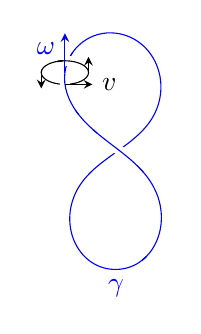
\begin{tikzpicture}[use Hobby shortcut]
	\begin{knot}[
 	 	consider self intersections=true,
 	 	%draft mode=crossings,
 		ignore endpoint intersections=false,
 		flip crossing=5,
	]
		\strand[blue] ([closed]0,0) .. (0.5,1) .. (-0.5,2) .. (-0.65,2.5) .. (0,3) .. (0.5,2) .. (-0.5,1) ..  (0,0);
		\strand (-0.65,2.5) circle[x radius=0.3, y radius=0.15];
	\end{knot}
	\draw[blue,-stealth](-0.65,2.5)--(-0.65,3) node[anchor=north east]{$\omega$};
	\draw[black,-stealth](-0.65,2.35)--(-0.3,2.35) node[anchor= west]{$v$};
	\draw[black,-stealth](-0.95,2.5)--(-0.95,2.3) node[anchor= west]{};
	\draw[black,-stealth](-0.35,2.5)--(-0.35,2.7) node[anchor= west]{};
	\node[blue,anchor= north] at (0,0) {$\gamma$};
\end{tikzpicture}
\end{document}

